The original SIR-model by Kermack-McKendrick \cite{SIR-model} can be formulated as follows describes how an infection is spread in a population consisting of three species: the number of susceptibles $S(t)$, the number of infectives $I(t)$ and the removed class $R(t)$ at time $t$. The model is given by

\begin{equation}
  \begin{split}
    \dv{S}{t}&=-rSI,\\
    \dv{I}{t}&=rSI-aI,\\
    \dv{R}{t}&=aI,\\
    \end{split}
  \label{eq:SIR}
\end{equation}
where $r>0$ is the infection rate and $a>0$ is the removal rate of infectives. Although this model looks like it has three states, qualitatively the state $R(t)$ can be viewed as a ``dummy state'' as the last ODE in Equation \eqref{eq:SIR} is independent of $R$. This means that we remove the third ODE without loosing any qualitative behaviour, and thereby reduce the above system to a two state system. From a symmetry perspective, the removal of the state $R$ would corresponds to $R$-autonomy implying that we have translations in $R$ in the same way as the model has a manifest time autonomy corresponding to translations in $t$. The qualitative behaviour of the SIR-model is restricted to the $SI$-phase plane.

The ODE describing the dynamics in the $SI$-phase plane is given by

\begin{equation}
\dv{I}{S}=\dfrac{rS-a}{rS}=\dfrac{a}{rS}-1
\label{eq:SI_phase_plane}
\end{equation}
and the reaction term can be considered separable with $g(I)=1$ and $f(S)=(rS-a)/rS$. As can be seen from Equation \eqref{eq:SI_phase_plane}, we have $I$-autonomy in the $SI$-phase plane, and by Theorem \ref{thm:separable} the non-trivial $S$-directional symmetry is given by $X=(rS/(rS-a))\partial_S$. In summary, the symmetries of the SIR-model are generated by the following infinitesimal generators of the Lie group
\begin{align} X_0&=\partial_t-rSI\partial_S+\left(rSI-aI\right)\partial_I+aI\partial_R\label{eq:SIR_0},\\
  X_t&=\partial_t\label{eq:SIR_t},\\
  X_S&=\left(\dfrac{rS}{rS-a}\right)\partial_S\label{eq:SIR_S},\\
  X_I&=\partial_I\label{eq:SIR_I},\\
  X_R&=\partial_R\label{eq:SIR_R}.
\end{align}
Here, the non-trivial generators $X_t$, $X_I$ and $X_R$ corresponds to translations. The symmetry generated by $X_S$ cannot be explicitly formulated, but we can write it down implicitly in terms of its canonical coordinates:
\begin{equation}
  \Gamma^{\mathrm{SIR},S}_{\epsilon}:(s,r_1,r_2,r_3)\mapsto(s+\epsilon,r_1,r_2,r_3),\quad s=S-\rho\ln\left(S\right),r_1=\tau,r_2=I,r_3=R,\rho=\dfrac{a}{r}\\
  \label{eq:SIR_S_symmetry}
\end{equation}
and the transformed coordinate $\hat{S}$ can be found by numerically solving
\begin{equation}
  S-\rho\ln\left(S\right)+\epsilon=\hat{S}-\rho\ln\left(\hat{S}\right)
  \label{eq:SIR_S_symmetry_numerics}
\end{equation}
for given values of $S$ and $\epsilon$ respectively. Moreover, the solution trajectories in the $(I,S)$-phase plane are readily calculated by integrating the ODE in Equation \eqref{eq:SI_phase_plane} with respect to $S$ and these are given by the following equation \cite{murray2002}

\begin{equation}
  I(S)=H_{\mathrm{SIR}}-(S-\rho\ln(S)),\quad H_{\mathrm{SIR}}=I_0+S_0-\rho\ln(S_0),\quad\rho=\dfrac{a}{r}
  \label{eq:SIR_trajectory}
\end{equation}
where the initial conditions in the $(I,S)$-phase plane are denoted by $I_0$ and $S_0$ respectively. Interestingly enough, we can express the transformed solution curve $\hat{I}(S;\epsilon)$ obtained by transforming the original solution curve $I(S)$ in Equation \eqref{eq:SIR_trajectory} by the symmetry $\Gamma^{\mathrm{SIR},S}_{\epsilon}$ in Equation \eqref{eq:SIR_S_symmetry}

\begin{equation}
\hat{I}(S;\epsilon)=(H_{\mathrm{SIR}}+\epsilon)-(S-\rho\ln(S)),\quad H_{\mathrm{SIR}}=I_0+S_0-\rho\ln(S_0),\quad\rho=\dfrac{a}{r}.
  \label{eq:SIR_transformed_trajectory}
\end{equation}
In fact, this transformed solution curve gives us an interpretation of the meaning of the symmetry transformations of $\Gamma^{\mathrm{SIR},S}_\epsilon$. The solution curve $I(S)$ in Equation \eqref{eq:SIR_trajectory} has a maximum point corresponding to the maximum number of infected in the population, and this value is important to know as it indicates how severe the epedemic will be. This maximum is obtained by the following point in the $(S,I)$-phase plane \cite{murray2002}
\begin{equation}
    (S,I)=(\rho,I_{\max}),\quad\rho=\dfrac{a}{r},\quad I_{\max}=H_{\mathrm{SIR}}-\left(\rho-\rho\ln\left(\rho\right)\right).
\label{eq:SIR_maxima}
  \end{equation}
Now, the transformed solution curve in Equation \eqref{eq:SIR_transformed_trajectory} implies that for each transformation with a transformation parameter of $\epsilon$, the value of the constant $H_{\mathrm{SIR}}$ increases from $H_{\mathrm{SIR}}$ to $H_{\mathrm{SIR}}+\epsilon$. In turn, this implies that the \textit{maximum number of infected individuals} $I_{\max}$ in Equation \eqref{eq:SIR_maxima} also increases from $I_{\max}$ to $I_{\max}+\epsilon$. Thus, for the SIR-model the transformation parameter $\epsilon$ of the symmetry $\Gamma^{\mathrm{SIR},S}_{\epsilon}$ can be interpreted as the increase in the \textit{maximum number of infected individuals} $I_{\max}$ which is clearly illustrated when the symmetry acts on solution trajectories in the $(S,I)$-phase plane (Fig \ref{fig:SIR_symmetry}). 


\begin{figure}[htbp!]
  \begin{center}
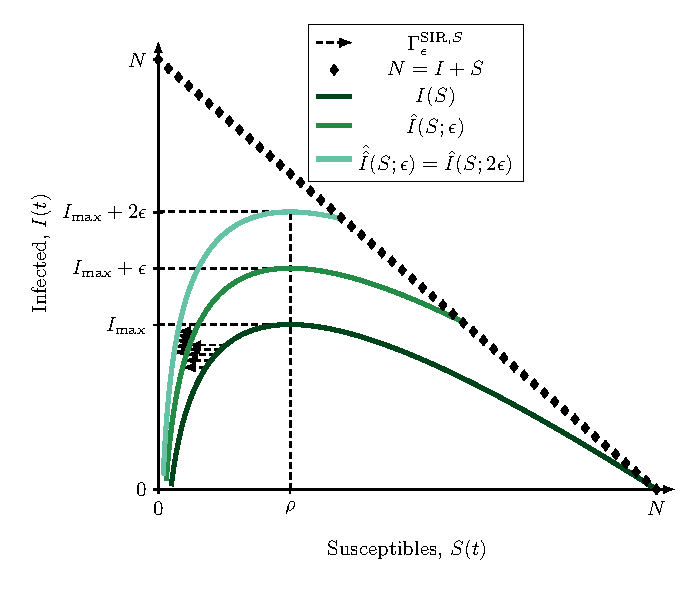
\includegraphics[width=\textwidth]{SIR_symmetry}
\caption{\textit{The $S$-directional symmetry of the SIR-model}. The $S$-directional symmetry $\Gamma^{\mathrm{SIR},S}_{\epsilon}$ of the SIR-model transforms the original $(S,I)$-curve in dark green with a transformation parameter of $\epsilon=200$ in order to obtain the transformed curve denoted by $(\hat{S},I)$ in light green. The parameters of the original solution curve are $N=763\;\mathrm{individuals}$, $r=0.00218\;\mathrm{days}^{-1}$, $\rho=a/r=202\;\mathrm{individuals}$, $S_0=762\;\mathrm{individuals}$ and $I_{\max}=292\;\mathrm{individuals}$. In particular, for each transformation by $\Gamma^{\mathrm{SIR},S}_{\epsilon}$ of the original solution curve by a transformation parameter $\epsilon$, the \textit{maximum number of infected individuals} $I_{\max}$ increases from $I_{\max}$ to $I_{\max}+\epsilon$. }
\label{fig:SIR_symmetry}
\end{center}
\end{figure}


